\documentclass{report}

\usepackage[utf8]{inputenc}
\usepackage[a4paper,includeheadfoot,margin=2.54cm, top=0.5in, bottom=0.5in]{geometry}
\usepackage{xcolor, hyperref, lipsum, graphicx}
\usepackage{amsmath, amsthm, amsfonts, textgreek}
\usepackage{listings}
\usepackage{color}
\usepackage{textcomp}
\usepackage{xinttools}
\usepackage{color}
\usepackage{listings}
\usepackage{caption, float}
\usepackage[most]{tcolorbox}
\usepackage{physics}
\usepackage{pifont}

\captionsetup[lstlisting]{skip=7pt}
\renewcommand\lstlistingname{Code}
\renewcommand\lstlistlistingname{Code}

\definecolor{darkred}{rgb}{0.6,0.0,0.0}
\definecolor{darkgreen}{rgb}{0,0.50,0}
\definecolor{lightblue}{rgb}{0.0,0.42,0.91}
\definecolor{orange}{rgb}{0.99,0.48,0.13}
\definecolor{grass}{rgb}{0.18,0.80,0.18}
\definecolor{pink}{rgb}{0.97,0.15,0.45}

\definecolor{mygreen}{rgb}{0,0.6,0}
\definecolor{mygray}{rgb}{0.5,0.5,0.5}
\definecolor{mymauve}{rgb}{0.58,0,0.82}


\lstset{language=java,
aboveskip=1em,
breaklines=true,
abovecaptionskip=-6pt,
frame=single,
numbers=left,
numbersep=15pt,
numberstyle=\tiny,
backgroundcolor=\color{white},   % choose the background color
basicstyle=\footnotesize,        % size of fonts used for the code
breaklines=true,                 % automatic line breaking only at whitespace
captionpos=b,                    % sets the caption-position to bottom
commentstyle=\color{mygreen},    % comment style
escapeinside={\%*}{*)},          % if you want to add LaTeX within your code
keywordstyle=\color{blue},       % keyword style
stringstyle=\color{mymauve},     % string literal style
}


\usepackage{fancyvrb}
\usepackage{fancyhdr, lastpage}
\pagestyle{fancyplain}% <- pagestyle fancyplain
\renewcommand\plainheadrulewidth{.4pt}% headrule on plain pages
\lhead{SAE 1.02}
\rhead{S1 - Renaud \& Franceus-Cointrel}
\cfoot{Page \thepage\ of \pageref{LastPage}}
\usepackage{setspace}
\onehalfspacing


\usepackage{titlesec}


\titlespacing*{\section}
{0pt}{5.5ex plus 1ex minus .2ex}{4.3ex plus .2ex}
\titlespacing*{\subsection}
{0pt}{5.5ex plus 1ex minus .2ex}{4.3ex plus .2ex}

\title{\textbf{SAE 1.02 - E3CETE}}
\author{J. Renaud - M. Franceus-Cointrel}
\date{Pour le 14 janvier 2024}


\addtolength{\jot}{1em}

\hypersetup{
  pdftitle={SAE 1.02 : E3Cete - 2023/2024},
  pdfauthor={Renaud Julien, Franceus-Cointrel Milwenn},
  pdfsubject={Dev. Init.}
}

\renewcommand{\contentsname}{Table des matières}
\renewcommand{\appendixname}{Annexe}
\renewcommand{\chaptername}{Chapitre}


\begin{document}

\maketitle
\tableofcontents

\chapter*{Introduction}

\qquad Dans cette SAE 1.02 nous étudions les \textit{Paquet} de \textit{Carte}. Un \textit{Paquet} est une collection de \textit{Carte} tous distincts. Une \textit{Carte} est définie par ses caractéristiques possibles, ici : \textit{Couleur}, \textit{nbFiguresMax}, \textit{Figure} et \textit{Texture}. 

\begin{figure}[H]
\centering
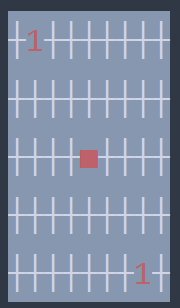
\includegraphics[scale=1]{../graphe/carte.png}
\caption{Affichage d'une carte \textit{ROUGE} ayant \textit{1} \textit{CARRE} et une texture \textit{LIGNES\_CROISEES}}
\end{figure}


\noindent En utilisant des outils informatiques, nous étudions des concepts mathématiques via la génération, le calcul, le stockage, le traitement, et l'affichage de données expérimentales ; pour les analyser et les comparer dans la mesure du possible aux valeurs théoriques. D'une part, nous nous intéressons au tri d'un \textit{Paquet} mélangé ; et d'autre part aux probabilités. Nous nous focaliserons en particulier sur 3 algorithmes de tris en place : le tri par séléction, le tri par insertion et le tri à bulles. Nous étudions également les probabilités de 3 événements particuliers : 3CR, 3CR\&2CL et E3C. 

\begin{figure}[H]
\centering
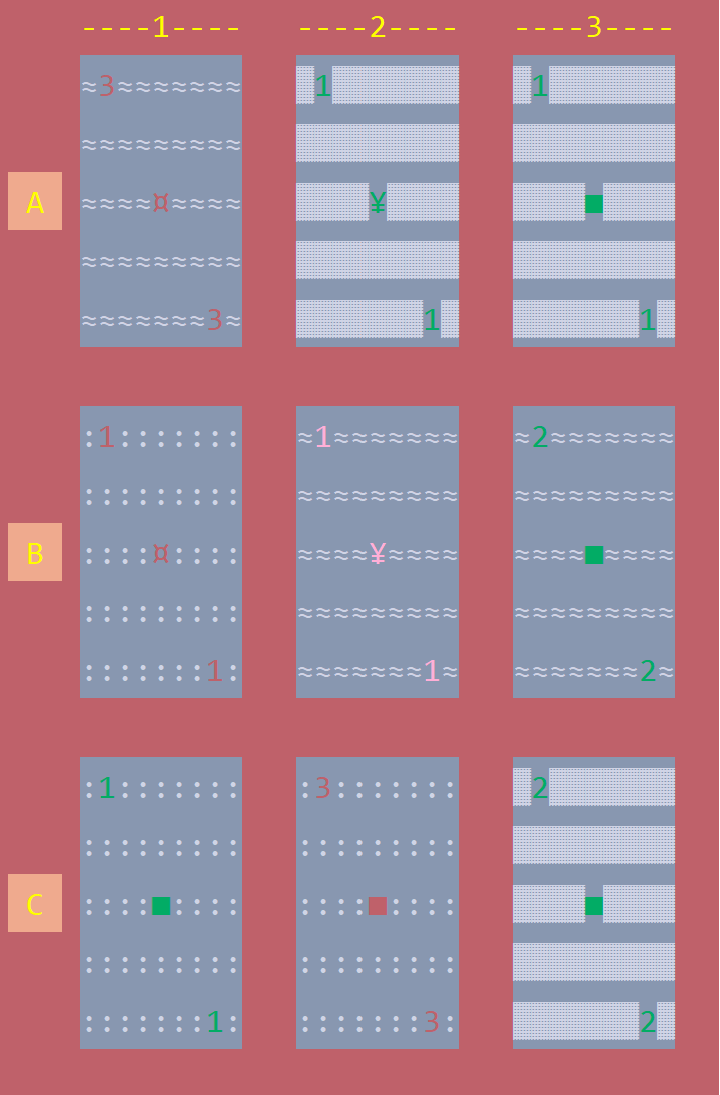
\includegraphics[scale=0.6]{../graphe/table.png}
\caption{Affichage d'une \textit{Table} 3x3 de \textit{Carte} de notre jeu E3C (paramètres par default)}
\end{figure}


\chapter{Analyse et comparaison des 3 méthodes de tris}

\qquad 

\section{Fonctions de tris et comptage du nombre d'opérations}

\qquad Afin d'étudier la performance des 3 méthodes de tris, nous devons compter approximativement le nombre d'opération élémentaire effectués lors d'un tel tri. Pour cela, nous utilisons une variable de \textit{Class} (globale) $nbOpApprox$ que nous initialisons à 0 au début de chaque tri. Nous incrémentons cette valeur de 1 pour chaque opération élémentaire réalisé lors du tri (affectation, condition, lecture...). Nous décidons d'omettre les opérations liées à l'incrémentation de $nbOpApprox$. Cela importe peu puisque ce qui nous intéresse est l'ordre de grandeur de la valeur $nbOpApprox$.

\subsection{Tri par sélection}

\begin{lstlisting}[language=java, caption={\it Fonction tri sélection}, label=codeSEL]
public Paquet trierSelection() {
    Paquet paqTri = new Paquet(this);
    nbOpApprox = 0;

    for (int i = 0; i < paqTri.nbCartesLeft-1; i++) {
        int indiceMin = i;
        for (int j = i+1; j < paqTri.nbCartesLeft; j++) {
            if (paqTri.cartes[j].compareTo(paqTri.cartes[indiceMin]) < 0) {
                indiceMin = j;
                nbOpApprox += 1; // 1 pour l'affectation
            }
            nbOpApprox += 4 + 6 + 1 ; //4 pour le for, 6 pour le compareTo, 1 pour le if
        }
        paqTri.swap2Cartes(i, indiceMin);
        nbOpApprox += 4 + 4 + 1; // 4 pour le swap, 4 pour le for, 1 pour l'affectation
    }
    return paqTri;
}
\end{lstlisting}

\subsection{Tri par propagation}

\begin{lstlisting}[language=java, caption={\it Fonction tri à bulles}, label=codeBUL]
public Paquet trierBulles() {
    Paquet paqTri = new Paquet(this);
    boolean inOrder = false;
    nbOpApprox = 1;
    while (!inOrder) {
        inOrder = true;
        for (int i = 0; i < paqTri.nbCartesLeft - 1; i++) {
            if (paqTri.cartes[i+1].compareTo(paqTri.cartes[i]) < 0) {
                paqTri.swap2Cartes(i+1, i);
                inOrder = false;
                nbOpApprox += 1 + 5; // 1 pour l'affectation, 5 pour le swap
            }
            nbOpApprox += 4 + 6 + 2; // 4 pour le for, 6 pour le compareTo, 2 pour le if
        }
        nbOpApprox += 2; // 2 pour le while
    }
    return paqTri;
}
\end{lstlisting}

\subsection{Tri par insertion}

\begin{lstlisting}[language=java, caption={\it Fonction tri insertion}, label=codeINS]
public Paquet trierInsertion() {
    Paquet paqTri = new Paquet(this);
    nbOpApprox = 0;
    for (int i = 1; i < paqTri.nbCartesLeft; i++) {
        int j = i;
        while (j > 0 && paqTri.cartes[j].compareTo(paqTri.cartes[j-1]) < 0) {
            paqTri.swap2Cartes(j, j-1);
            j--;
            nbOpApprox += 6 + 2 + 1 + 5; // 6 pour le compareTo, 2 pour le while, 1 pour l'affectation, 5 pour le swap
        }
        nbOpApprox += 4 + 6 + 2; // 4 pour le for, (6+2) pour le while dans la cas on ne rentre pas
    }
    return paqTri;
}
\end{lstlisting}

\pagebreak



\section{Protocole de test}

\subsection{Définition des variables}

L'objectif de cette expérience est d'évaluer la performance de chacun des tris. Pour cela nous devons réaliser chacun des tris en variant le nombre de cartes $N$ contenus dans le Paquet. Pour cette expérience les paquets triés seront toujours pleins, et le nombre de cartes $N$ contenus est déterminé par les cardinalités des caractéristiques possibles. En principe nous fixons les cardinalités associés aux couleurs/figures/textures pour ne seulement varier le nombres de répétition des figures. Ainsi le nombre de cartes $N$ est défini tel que : 

\begin{equation*}
	N = cardCouleurs \times cardFigures \times cardTextures \times cardRepetFigures
\end{equation*}

\bigskip

\noindent Pour chacune des méthodes de tris nous calculons le nombre d'opération $nOpApprox$ et son temps d'éxecution (en ms) $tempsExec$. Ainsi, en répétant les tris $nbRepetTest$ nombre de fois pour $N$ fixé, nous en déduisions les valeurs moyennes ainsi que leurs incertitudes (écartype) telles que :

\boldmath
\begin{equation} \label{eq:1}
nbOpMoy = \dfrac{1}{nbRepetTest} \times \sum_{i = 1}^{nbRepetTest} nbOpApprox_{i}
\end{equation} 
\begin{equation} \label{eq:2}
	u\_nbOp = \sqrt{\dfrac{1}{nbRepetTest} \times \sum_{i = 1}^{nbRepetTest} (\,nbOpApprox_{i} - nbOpMoy)\,^{2}}
\end{equation} 
\begin{equation} \label{eq:3}
	tempsExecMoy = \dfrac{1}{nbRepetTest} \times \sum_{i = 1}^{nbRepetTest} tempsExec_{i}
\end{equation} 
\begin{equation} \label{eq:4}
	u\_tempsExec = \sqrt{\dfrac{1}{nbRepetTest} \times \sum_{i = 1}^{nbRepetTest} (\,tempsExec_{i} - tempsExecMoy)\,^{2}}
\end{equation} 
\unboldmath

\subsection{Protocole expérimental}

\begin{enumerate}
	\item Réaliser les 3 tris sur $nbRepetTest$ paquets ayant les mêmes caractéristiques mais chacun mélangés différemment, pour un même nombre de cartes $N$.
	\item Récupérer le nombre d'opération $nbOpApprox$ et le temps d'éxécution $tempsExec$ de chacun des tris pour toutes les répétitions.
	\item Calculer et stocker les valeurs moyennes $nbOpMoy$ (\ref{eq:1}) et $tempsExecMoy$ (\ref{eq:3}), ainsi que leurs incertitudes $u\_nbOp$ (\ref{eq:2}) et $u\_tempsExec$ (\ref{eq:4}).
	\item Répéter l'expérience en variant $N$, en modifiant la valeur de $cardRepetFigures$.
\end{enumerate}

\pagebreak
\subsection{Code associé au protocole}

\begin{lstlisting}[language=java, caption={\it Fonctions de calculs de données expérimentales}, label=codeTRI]

/**
 * FONCTION AJOUTEE
 * Action : realise les 3 methodes de tris pour un paquet initialise a nbCartes nombre de carte.
 * Pour cette fonction le nombre de Couleur/nbFigures/Figure/Texture sont fixes (variables de classes : cardCouleurs, cardRepetFigures, cardFigures, cardTextures).
 * Nous repetons ces tris plusieurs fois (valeurs entres en params) sur des paquets presentant les memes caracteristiques mais melanges differremment ; pour obtenir des donnees significatifs :
 * Stock les donees relatifs (nb Cartes, nombre OP et temps exec) aux tris dans un tableau de tableau.
 * tabInfos[O a 2][0] --> nbCartes
 * tabInfos[O a 2][1] --> nbOP moyen
 * tabInfos[O a 2][2] --> ecart-type nbOp
 * tabInfos[O a 2][3] --> tempsExec moyen
 * tabInfos[O a 2][4] --> ecart-type tempsExec
 * 
 * tabInfos[0][0 a 4] --> Infos de Methode SELECTION
 * tabInfos[1][0 a 4] --> Infos de Methode BULLES
 * tabInfos[2][0 a 4] --> Infos de Methode INSERTION
 * @param nbRepetition
 * @return un tableau de tableau (3x3) de double.
 */
private static double[][] trisPaquet(int nbRepetition) {
    double[][] tabInfos = new double[3][5];
    double tempsExec;
    double[][][] tabInterm = new double [3][2][nbRepetition];

    Paquet paq;

    for (int i = 0; i < nbRepetition; i++) {
        paq = new Paquet(
            Couleur.valuesInRange(0, cardCouleurs), 
            cardRepetFigures, 
            Figure.valuesInRange(0, cardFigures), 
            Texture.valuesInRange(0, cardTextures)
            );

        tempsExec = Ut.getTempsExecution(paq::trierSelection);
        tabInterm[0][0][i] = nbOpApprox;
        tabInterm[0][1][i] = tempsExec;

        tempsExec = Ut.getTempsExecution(paq::trierBulles);
        tabInterm[1][0][i] = nbOpApprox;
        tabInterm[1][1][i] = tempsExec;

        tempsExec = Ut.getTempsExecution(paq::trierInsertion);
        tabInterm[2][0][i] = nbOpApprox;
        tabInterm[2][1][i] = tempsExec;   
    }

    for (int i = 0; i < 3; i++) {
        tabInfos[i][0] = cardCouleurs * cardRepetFigures * cardFigures * cardTextures;
    }
    tabInfos[0][1] = Ut.moyenne(tabInterm[0][0]);
    tabInfos[0][2] = Ut.ecarttype(tabInterm[0][0]);
    tabInfos[0][3] = Ut.moyenne(tabInterm[0][1]);
    tabInfos[0][4] = Ut.ecarttype(tabInterm[0][1]);
    
    tabInfos[1][1] = Ut.moyenne(tabInterm[1][0]);
    tabInfos[1][2] = Ut.ecarttype(tabInterm[1][0]);
    tabInfos[1][3] = Ut.moyenne(tabInterm[1][1]); 
    tabInfos[1][4] = Ut.ecarttype(tabInterm[1][1]);

    tabInfos[2][1] = Ut.moyenne(tabInterm[2][0]);
    tabInfos[2][2] = Ut.ecarttype(tabInterm[2][0]);
    tabInfos[2][3] = Ut.moyenne(tabInterm[2][1]); 
    tabInfos[2][4] = Ut.ecarttype(tabInterm[2][1]);

    return tabInfos;
}

/**
 * FONCTION AJOUTEE
 * Prerequis : 0 < nStart < nEnd ET 0 < nStep 
 * Action : realise trisPaquet(int nbRepetition) en variant le nbCartes en modifiant la cardinalite de nbFigures, entre en parametres, de nStart a nEnd(exclu) en faisant des pas de nStep.
 * Les cardinalites de couleurs/figures/textures sont fixees a des valeurs constantes par les variables de class.
 * @param nStart premiere valeur de nbFiguresMax
 * @param nEnd valeur limite (exclue)
 * @param nStep pas
 * @return un tableau contenant tout les resultats de chacun des trisPaquet().
 */
private static double[][][] testTrisVarN(int nStart, int nEnd, int nStep) {
    int range = (int) Math.ceil((float) (nEnd - nStart)/nStep);
    double[][][] tabInfos = new double[range][3][5];
    int count = 0;
    
    for (int n = nStart; n < nEnd; n+=nStep) {
        cardRepetFigures = n;
        tabInfos[count] = trisPaquet(nbRepetTest);
        count++;
    }
    return tabInfos;
}
\end{lstlisting}



\newpage
\section{Tests}
\subsection{Initialisation et spécificités}
Les variables :
\begin{itemize}
	\item int $nbRepetTest = 1000$
	\item int $cardCouleurs = 1$ ; int $cardFigures = 1$ ; int $cardTextures = 1$
	\item Test 1 : int $cardRepetFigures \in [\, 10-500 ]\, $ ; step = 1
	\item Test 2 : int $cardRepetFigures \in [\, 1000-10 000 ]\, $ ; step = 1000
	
\end{itemize}
Specificités de l'appareil utilisés :
\begin{itemize}
	\item[\ding{228}] CPU : 12th Gen Intel(R) Core(TM) i5-1240P   1.70 GHz
	\item[\ding{228}] RAM : 16.0 GB
	\item[\ding{228}] OS  : Windows 11
\end{itemize}



\subsection{Analyse graphique}

\qquad Nous stockons les données des tests sous forme de fichier .csv, grâce à une fonction de conversion. Le fichier contient les informations des 3 tris, i.e. toutes les valeurs de $N$, $nbOpMoy$, $u\_nbOp$, $tempsExec$, $u\_tempsExec$ pour chacune des méthodes de tri. 

\begin{figure}[H]
	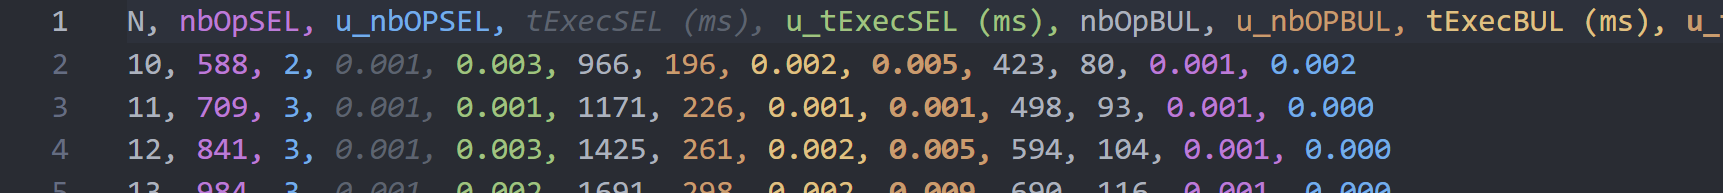
\includegraphics[width=\textwidth]{../graphe/csvEx.png}
	\caption{Exemple de données dans le fichier .csv en question}
\end{figure}

\begin{enumerate}
	\item[\fcolorbox{black}{black}{\textbf{\textcolor{white}{3}}}] 
	Nous choisissons de réaliser le graphique de $nbOpMoy=f(\,N)\,$ et de $tempsExecMoy=f(\,N)\,$ à l'aide du logiciel \href{https://regressi.fr/WordPress/}{\it \underline{Regressi}}. Etant donées que ces 3 fonctions de tris utilisent chacune une double boucle imbriquée, nous nous attendons à une complexité quadratique $O(\,n^2\,)$.
\end{enumerate}
\qquad Nous observons bien sur les graphiques ci-dessous une compléxité quadratique, puisque les courbes s'apparentent à des paraboles. Quant à la performance de ces 3 tris en place, le Tri à bulles est le moins performant et le moins stable (incertitudes qui augmentent avec $N$) ; ce qui est cohérent puisque ce-dernier compare répétitivement les cartes "consécutifs" du Paquet, et les permutent si "non triées". Ainsi, pour un paquet désordonné il réalise beaucoup de permutations de cartes. Ensuite, le Tri par sélection semble être le plus stable. Ceci s'explique du fait que pour un même $N$, il réalise toujours le même nombre d'opération et permutations quelque soit l'arrangement du Paquet. Finalement, le tri par Insertion est celui qui est le plus rapide (du moins pour $N<500$). En effet, ce dernier est efficace lorsque le Paquet est partiellement trié, puisque pour chacune des cartes, il consiste à le placer au bon endroit dans le tableau parmi toutes les cartes précédentes qui sont déjà ordonnées. D'ailleurs, nous observons que pour $N$ plus importants (Test n°2) le tri par séléction l'emporte sur  le tri par insertion au niveau du temps d'éxecution. Nous avons choisi de réaliser un deuxième test pour $N$ plus élevés pour avoir des valeurs plus significatifs concernant le temps d'éxécution.

\subsection{Graphiques : Test 1}

\begin{figure}[H]
	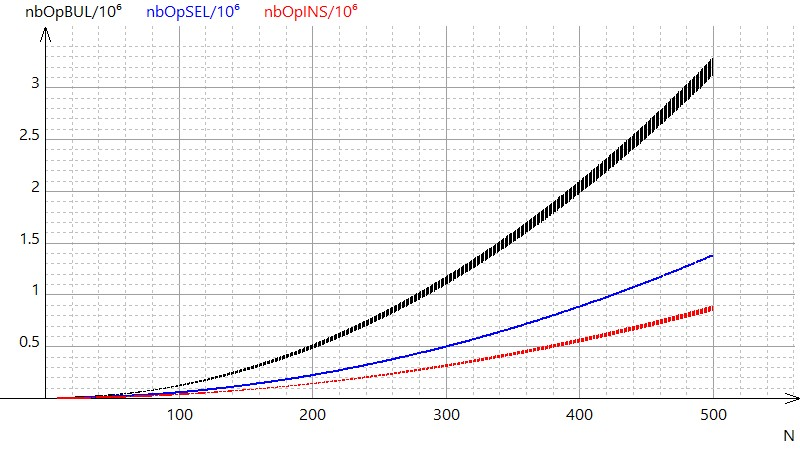
\includegraphics[width=\textwidth]{../graphe/nbOp.jpg}
	\label{nbOP1}
	\caption{Graphique de $nbOpMoy=f(\,N)\,$ avec les barres d'incertitudes sur $nbOpMoy$ pour les 3 méthodes de tris : en noir le tri à bulles, en bleu le tri sélection et en rouge le tri insértion.}
\end{figure}
\begin{figure}[H]
	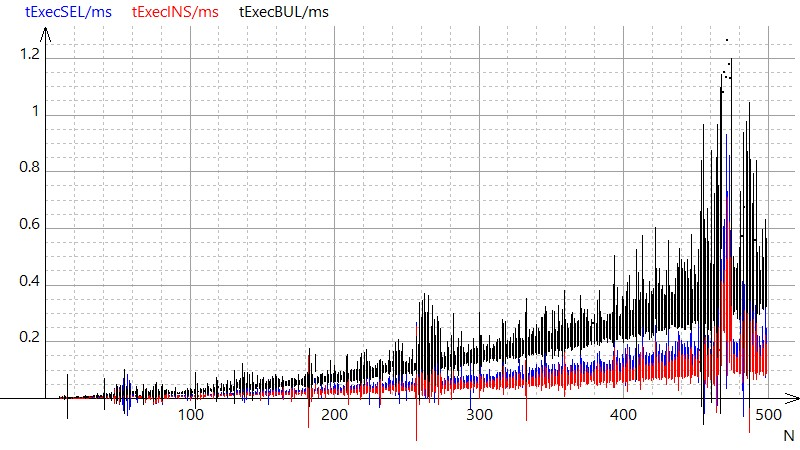
\includegraphics[width=\textwidth]{../graphe/tExecAvecU.jpg}
	\label{tExec1}
	\caption{Graphique de $tempsExecMoy=f(\,N)\,$ avec les barres d'incertitudes sur $tempsExecMoy$ pour les 3 méthodes de tris : en noir le tri à bulles, en bleu le tri sélection et en rouge le tri insértion.}
\end{figure}

\subsection{Graphiques : Test 2}

\begin{figure}[H]
	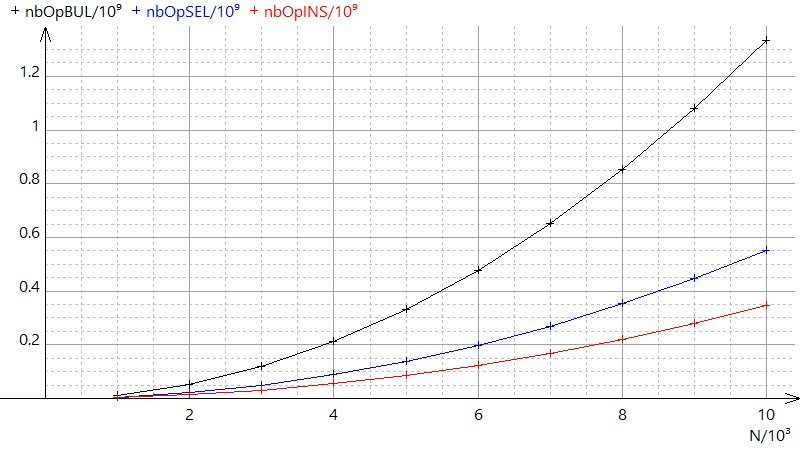
\includegraphics[width=\textwidth]{../graphe/nbOP10a10k.jpg}
	\label{nbOP1k}
	\caption{Graphique de $nbOpMoy=f(\,N)\,$ avec les barres d'incertitudes sur $nbOpMoy$ pour les 3 méthodes de tris : en noir le tri à bulles, en bleu le tri sélection et en rouge le tri insértion.}
\end{figure}
\begin{figure}[H]
	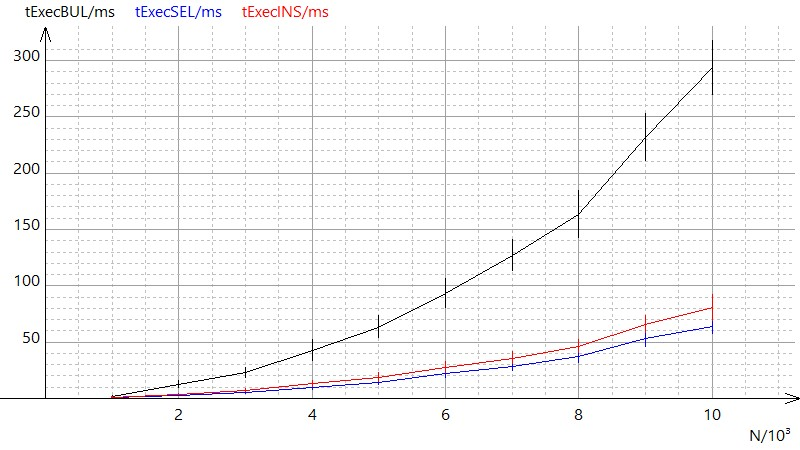
\includegraphics[width=\textwidth]{../graphe/tExec10a10k.jpg}
	\label{tExec1k}
	\caption{Graphique de $tempsExecMoy=f(\,N)\,$ avec les barres d'incertitudes sur $tempsExecMoy$ pour les 3 méthodes de tris : en noir le tri à bulles, en bleu le tri sélection et en rouge le tri insértion.}
\end{figure}






\newpage
\chapter{Théorie}

\section{Représentation mathématique de la Class \it Table}
\begin{enumerate}
	\item[\fcolorbox{black}{black}{\textbf{\textcolor{white}{4}}}] 
	En termes de structure de données, une \textit{Table} est un tableau de \textit{Carte}. Les \textit{Carte} d'une \textit{Table} sont indicés par rapport à leur position dans le tableau, ce qui détermine leurs positions sur la \textit{Table} au niveau de l'affichage graphique. Ainsi, une \textit{Table} est une liste ordonnée de \textit{Carte} tous différentes (pas de répétition), parmi toutes les \textit{Carte} du jeu contenues dans un \textit{Paquet}. Une \textit{Table} est donc un arrangement. 
	
	\item[\fcolorbox{black}{black}{\textbf{\textcolor{white}{5}}}] 
	Pour une \textit{Table} de 9 \textit{Cartes} et un jeu de 81 \textit{Cartes}, le nombre de \textit{Tables} différentes possibles est tel que : 
	\bigskip
	$$A^{9}_{81} = \frac{81!}{(81-9)!} = 81\times80\times...\times74\times73 = 94670977328928000$$
\end{enumerate}

\section{Démarche expérimental}
\qquad L'expérience consiste à répeter $nbEssai$ fois l'action suivante : piocher 9 cartes d'un paquet mélangé de 81 cartes. Nous obtenons sur la table un arrangement de ces 9 cartes. L'événement 3CR consiste à détecter si parmi ces 9 cartes, on a exactement 3 cartes rouges. L'événement 3CR\&2CL consiste à détecter si parmi ces 9 cartes, on a exactement 3 cartes rouges et 2 cartes ayant au moins un losange. L'événement E3C consiste à détecter si parmi ces 9 cartes, on a au moins un E3C.
\bigskip

\noindent Pour chacun de ces événements : \\
On notera $Freq$ la fréquence de cet evenement durant l'experience.
De la $Freq$ on en deduit la probabilité individuelle empirique $P$ de l'événement associé à cette experience : $P=\frac{Freq}{nbEssai}$.
De cela nous pouvons en déduire le pourcentage d'erreur $Erreur$ de cette probabilité par rapport à la valeur théorique calculée (si c'est le cas).
\bigskip

\noindent Ensuite, nous répétons l'experience en variant $nbEssai$, et nous regardons l'évolution de la $Freq$, de $P$ et de $Erreur$ en fonction de $nbEssai$.
\newpage
\begin{lstlisting}[language=java, caption={\it Fonction pour réaliser les expériences en variant nbEssai avec l'événement à choisir en paramètre}, label=codeProba]
/**
 * FONCTION AJOUTEE
 * Prerequis : 0 <= startEssai < endEssai ET 0 <= stepEssai 
 * experience = 1 pour probabilite de 3CR
 * experience = 2 pour probabilite de E3C
 * experience = 3 pour probabilite de E3C&2CL
 * Action : Realise les fonctions proba3CR(int nbEssai) ou probaE3C(int nb) en 
 * faisant varier le nombre d'essai de startEssai a endEssai en faisant des pas
 * de stepEssai.
 * Stock les donnees dans un tableau de double de taille 4 :
 *  tabStats[0] --> Nombre d'essai
 *  tabStats[1] --> Frequence de cas favorables de l'evenement
 *  tabStats[2] --> Probablilite individuelle : P = frequence/nbEssai
 *  tabStats[3] --> Pourcentage d'Erreur de la probabilite individuelle de l'evenement par rapport a la valeur theorique ; calculable seulement en connaissance de la valeur theorique
 * Convertion de ces donnees en String adaptes au format .csv et ecrit le String dans un fichier : "proba3CR.csv" ou "probaE3C.csv" ou "proba3CR&2L"
 */
public static void probaVarEssai(int startEssai, int endEssai, int stepEssai, int experience) throws FileNotFoundException {
    int range = (int) Math.ceil((float) (endEssai - startEssai)/stepEssai);
    double[][] tabStats = new double[range][4];
    int count = 0;
    for (int i = startEssai; i < endEssai; i+=stepEssai) {
        tabStats[count][0] = i;
        if (experience == 1) {
            tabStats[count][1] = proba3CR(i);
            tabStats[count][2] = tabStats[count][1]/i; //proba individuelle
            tabStats[count][3] = Ut.pourcentageErreur(0.28956680871386137, tabStats[count][2]); 
        }
        else if (experience == 2) {
            tabStats[count][1] = probaE3C(i);
            tabStats[count][2] = tabStats[count][1]/i; //proba individuelle
            //na calcul pas erreur car pas de val theorique
        }
        else if (experience == 3) {
            tabStats[count][1] = proba3CRAnd2CL(i);
            tabStats[count][2] = tabStats[count][1]/i; //proba individuelle
            tabStats[count][3] = Ut.pourcentageErreur(0.06884362550959248, tabStats[count][2]); 
        }
        count++;
    }
    if (experience == 1) {
        stringInfosToCsv(probaDatasToString(tabStats), "proba3CR"); 
    }
    else if (experience == 2) {
        stringInfosToCsv(probaDatasToString(tabStats), "probaE3C");
    }
    else if (experience == 3) {
        stringInfosToCsv(probaDatasToString(tabStats), "proba3CR&2L");
    }
}
\end{lstlisting}


\section{Etude du cas 3CR}
\subsection{Calculs théoriques}




\bigskip
\begin{enumerate}
	\item[\fcolorbox{black}{black}{\textbf{\textcolor{white}{6}}}] 
	Sachant que pour une \textit{Carte} il y a 3 \textit{Couleurs}, 3 répétitions maximales de figures, 3 \textit{Figures} et 3 \textit{Textures} possibles ; on en déduit qu'il existe $1\times3\times3\times3=27$ cartes rouges distinctes. Pour déterminer les arrangements possibles contenant exactement 3 cartes rouges : comme l'ensemble des cartes rouges et l'ensemble des cartes non rouges sont disjoints, nous comptons le nombre de combinaisons possibles de 3 cartes rouges parmi les 27 cartes rouges du paquet ; et le nombre de combinaisons possibles de 6 cartes non rouges parmi les $81 - 27 = 54$ cartes non rouges. A chacune de ces combinaisons possibles de 3 cartes rouges + 6 cartes non rouges (jusque là pas d'ordre), nous pouvons réaliser $9!$ permutations possibles (relation d'ordre). Ainsi, le nombre de \textit{Tables} différentes contenant exactement 3 \textit{Cartes} rouges est tel que :	
	$$C^{3}_{27} \times C^{6}_{81-27} \times 9! = \frac{27!}{3!(27-3)!} \times  \frac{54!}{6!(54-6)!} \times 9! = 2925 \times 25827165 \times 362880 = 27413572782960000$$

	\item[\fcolorbox{black}{black}{\textbf{\textcolor{white}{7}}}] 
	On en déduit la probabilité $P_{3CR}$ d'obtenir une \textit{Table} contenant exactement 3 cartes rouges :
	$$P_{3CR} = \dfrac{casFavorables}{casTotal} = \dfrac{C^{3}_{27} \times C^{6}_{81-27} \times 9!}{A^{9}_{81}} = \dfrac{27413572782960000}{94670977328928000} = 0.28956680871386137 $$
\end{enumerate}


\subsection{Fonction \textit{proba3CR}}


\begin{enumerate}
	\item [\fcolorbox{black}{black}{\textbf{\textcolor{white}{8}}}] 
	Fonction qui retourne le fréquence de l'événement 3RC parmi $nbEssai$ entré en paramètre.
\end{enumerate}

\begin{lstlisting}[language=java, caption={\it Fonction proba3CR}, label=codeProba3CR]
/**
 * FONCTION AJOUTEE
 * Action : Pour un paquet de 81 cartes distincts (3 Couleurs/ nbFiguresMax=3/ 3 Figures/ 3 Textures possibles par carte) : 
 * calcul experimentalement et retourne la frequence d'obtenir une Table (arrangement de 9 cartes distincts parmi les 81 du Paquet) contenant exactement 3 Cartes Rouges.
 * Valeur theorique : 0.28956680871386137
 * @param nbEssai nombre d'essai
 */
public static double proba3CR(int nbEssai) {
    double countCasFavorable = 0;
    Paquet paq;
    for (int j = 0; j < nbEssai; j++) {
        paq = new Paquet(
            Couleur.valuesInRange(0, 3), 
            3, 
            Figure.valuesInRange(0, 3), 
            Texture.valuesInRange(0, 3)
            );
        Carte[] tab = paq.piocher(9);
        double countRed=0;
        for (int k = 0; k < tab.length; k++) {
            if (tab[k].getCouleur() == Couleur.ROUGE) {
                countRed++;
            }
        }
        if (countRed==3) {
            countCasFavorable++;
        }
    }
    return countCasFavorable;
}
\end{lstlisting}



\subsection{Traitements de données et analyse graphique}
\begin{figure}[H]
	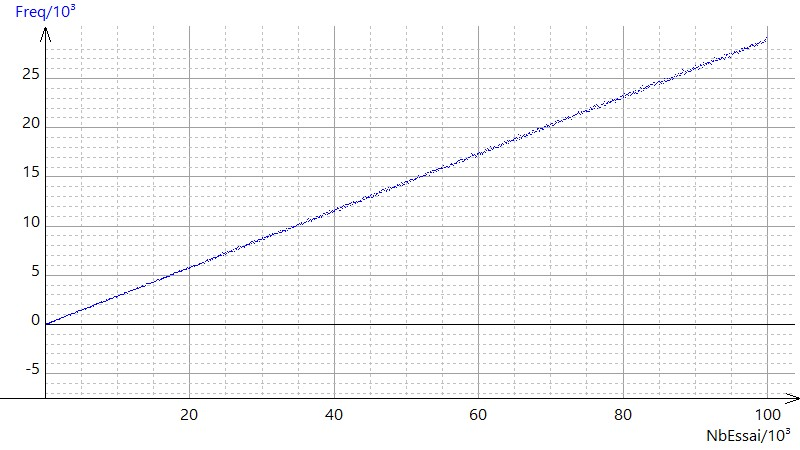
\includegraphics[width=\textwidth]{../graphe/Freq(n).jpg}
	\caption{Graphique de $Freq=f(nbEssai)$ en variant $nbEssai$ de 100 à 100 000 par pas de 100}
\end{figure}	
\bigskip

Les graphiques obtenus à partir des données générées par cette fonction permettent de déterminer une valeur expérimental de $P_{3CR}exp$. En effet, en traçant $Freq=f(nbEssai)$ nous apercevons que la courbe varie linéairement. Ceci est en accord avec la théorie puisque $P_{3CR}theo = \dfrac{casFavorables}{casTotal}$ soit $casFavorables = P_{3CR}\times casTotal$ ce qui équivaut à  $Freq=a\times nbEssai$. En réalisant une modélisation linéaire grâce à l'outils de modélisation sur le logiciel \href{https://regressi.fr/WordPress/}{\it \underline{Regressi}} ; nous en déduisons : 
$$P_{3CR}exp = a = 0.28939 \pm 0.00015$$
Nous pouvons calculer le pourcentage d'erreur $Err$ telle que :
$$Err = abs\left(\dfrac{P_{3CR}theo - P_{3CR}exp}{P_{3CR}theo}\right) \times100 = 0.061\%$$	

\newpage


\begin{figure}[H]
	\centering
	\includegraphics[scale=0.5]{../graphe/ValdeP.png}
	\caption{Modélisation linéaire de $Freq(nbEssai)$ sur \textit{Regressi}}
\end{figure}

\bigskip
\noindent Pour déterminer à partir de combien d'essais il faut pour obtenir un résultat fiable, nous avons choisi de tracer $Err=f(nbEssai)$ à partir des probabilités propres à chacun des événements (associé au nombre d'essais) : $P = Freq/nbEssai$.
\begin{figure}[H]
	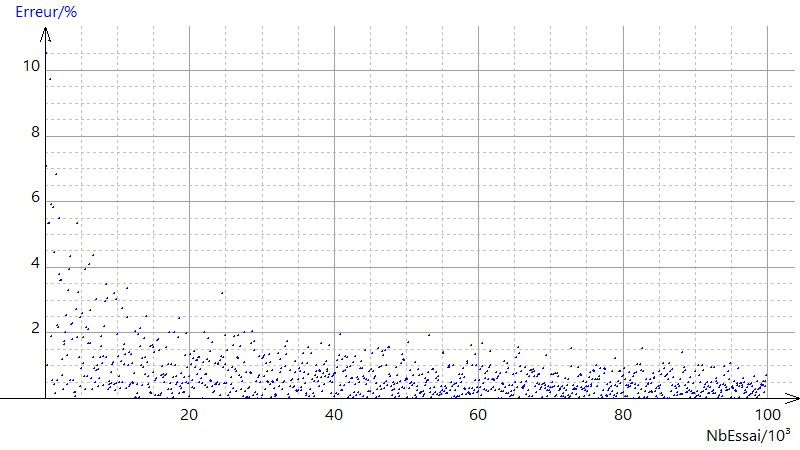
\includegraphics[width=\textwidth]{../graphe/Erreur(n).jpg}
	\caption{Graphique de $Erreur=f(nbEssai)$ en variant $nbEssai$ de 100 à 100 000 par pas de 100}
\end{figure}	
\noindent Nous observons que pour avoir un résultat fiable à 5\% d'erreur près, il faut au moins environ 10 000 essais. Le graphique ci-dessous de $P=f(nbEssai)$ illustre bien la répartition des probabibilités qui converge vers la valeur théorique en augmentant le nombre d'essais. 
\begin{figure}[H]
	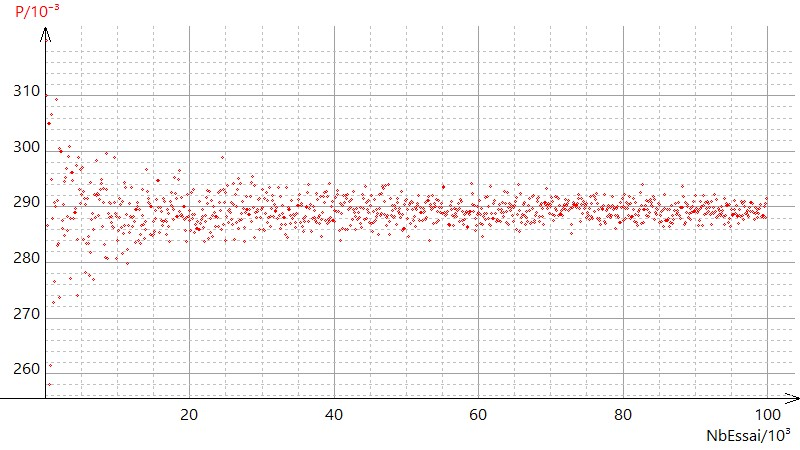
\includegraphics[width=\textwidth]{../graphe/P(n).jpg}
	\caption{Graphique de $P=f(nbEssai)$ en variant $nbEssai$ de 100 à 100 000 par pas de 100}
\end{figure}	


\section{Etude du cas 3CR\&2CL}

\subsection{Caluls théoriques}
\begin{enumerate}
	\item [\fcolorbox{black}{black}{\textbf{\textcolor{white}{8}}}] 
	L'intersection de l'ensemble des cartes rouges et des cartes ayant au moins un losange n'est pas vide. Il faut étudier chacun des cas et diviser les ensembles en ensembles disjoints. Il y a 27 cartes rouges distincts et 27 cartes ayant au moins un losange. Parmi ces cartes rouges seulement $1\times3\times2\times3=18$ n'ont pas de losange. De même, parmi les cartes ayant au moins un losange, $2\times3\times1\times3=18$ ne sont pas rouges. Ainsi, $1\times3\times1\times3=9$ cartes sont à la fois rouges et ont au moins un losange. 
\bigskip

\begin{table}[H]
\centering
\begin{tabular}{|c||c c c c||c|} 
 \hline
 Carte & R$\land$L & R$\land\neg$L & L$\land\neg$R & $\neg$(R$\lor$L) & SUM \\ [0.5ex] 
 \hline\hline
 Total & 9 & 18 & 18 & 36 & 81\\ 
 Cas 1 & 2 & 1 & 0 & 6 & 9 \\
 Cas 2 & 1 & 2 & 1 & 5 & 9 \\
 Cas 3 & 0 & 3 & 2 & 4 & 9\\[1ex] 
 \hline
\end{tabular}
\caption{Tableau récapitulatif des différents cas possibles pour obtenir une combinaison de 9 cartes avec exactement 3 cartes rouges (R) et 2 cartes ayant au moins un losange (L) :}
\end{table}

\newpage

On en déduit le nombre d'arrangements possibles de \textit{Table} contenant exactement 3 cartes rouges et 2 cartes ayant au moins un losange tel que :

\begin{align*}
9! &\times(\,C^{2}_{9} \times C^{1}_{18} \times C^{0}_{18} \times C^{6}_{36} \\
&+C^{1}_{9} \times C^{2}_{18} \times C^{1}_{18} \times C^{5}_{36} \\
&+C^{0}_{9} \times C^{3}_{18} \times C^{2}_{18} \times C^{4}_{36} )\, \\
&= 362880 \times 17960464368 = 6517493309859840
\end{align*}

On en déduit la probabilité $P_{3CR\&2CL}$ de cet événement :
	$$P_{3CR\&2CL} = \dfrac{casFavorables}{casTotal} = \dfrac{6517493309859840}{94670977328928000} = 0.06884362550959248 $$
\end{enumerate}

\subsection{Fonction \textit{proba3CR\&2CL}}


\begin{lstlisting}[language=java, caption={\it Fonction proba3CRAnd2CL}, label=codeProba3CR2L]
/**
 * FONCTION AJOUTEE
 * Action : Pour un paquet de 81 cartes distincts (3 Couleurs/ nbFiguresMax=3/ 3 Figures/ 3 Textures possibles par carte) : 
 * calcul experimentalement et retourne la frequence d'obtenir une Table (arrangement de 9 cartes distincts parmi les 81 du Paquet) contenant exactement 3 Cartes Rouges et 2 cartes ayant au moins 1 Losange.
 * Valeur theorique : 0.06884362550959248
 * @param nb nombre d'essai
 */
public static double proba3CRAnd2CL(int nb) {
    double countCasFavorable = 0;
    Paquet paq;
    for (int i = 0; i < nb; i++) {
        paq = new Paquet(
            Couleur.valuesInRange(0, 3), 
            3, 
            Figure.valuesInRange(0, 3), 
            Texture.valuesInRange(0, 3)
            );
        Carte[] tab = paq.piocher(9);
        double countRed=0;
        double countLosange=0;
        for (int j = 0; j < tab.length; j++) {
            if (tab[j].getCouleur() == Couleur.ROUGE) {countRed++;}
            if (tab[j].getFigure() == Figure.LOSANGE) {countLosange++;}
        }
        if (countRed==3 && countLosange==2) {
            countCasFavorable++;
        }
    }
    return countCasFavorable;
}
\end{lstlisting}




\subsection{Traitements de données et analyse graphique}

\noindent De la même manière que pour le cas 3CR, nous obtenons via une modélisation linéaire :

$$P_{3CR\&2CL}exp = 0.06883 \pm 0.00006$$
Nous pouvons calculer le pourcentage d'erreur $Err$ telle que :
$$Err = abs\left(\dfrac{P_{3CR\&2CL}theo - P_{3CR\&2CL}exp}{P_{3CR\&2CL}theo}\right) \times100 = 0.020\%$$	

\begin{figure}[H]
	\centering
	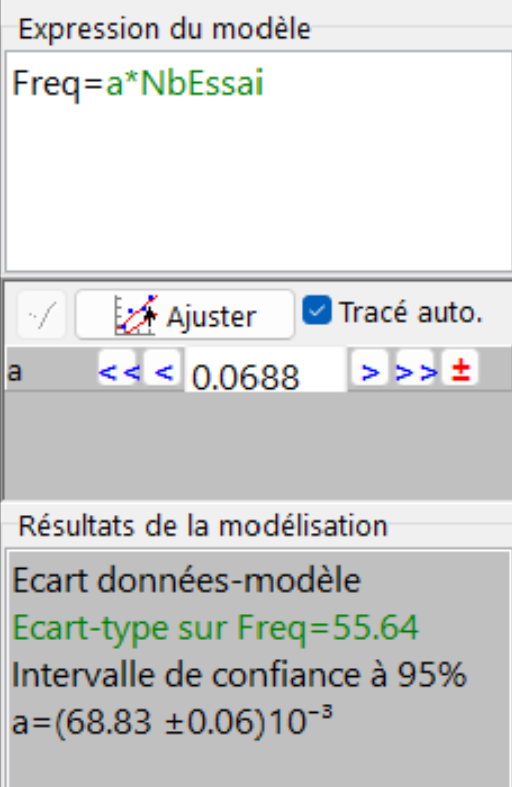
\includegraphics[scale=0.5]{../graphe/valDeP3CR2L.png}
	\caption{Modélisation linéaire de $Freq(nbEssai)$ sur \textit{Regressi}}
\end{figure}

\begin{figure}[H]
	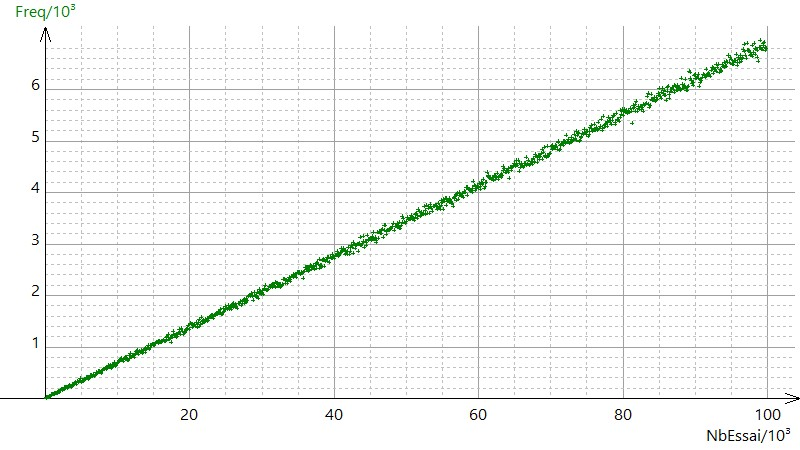
\includegraphics[width=\textwidth]{../graphe/Freq3CR2L(n).jpg}
	\caption{Graphique de $Freq=f(nbEssai)$ en variant $nbEssai$ de 100 à 100 000 par pas de 100}
\end{figure}	

\begin{figure}[H]
	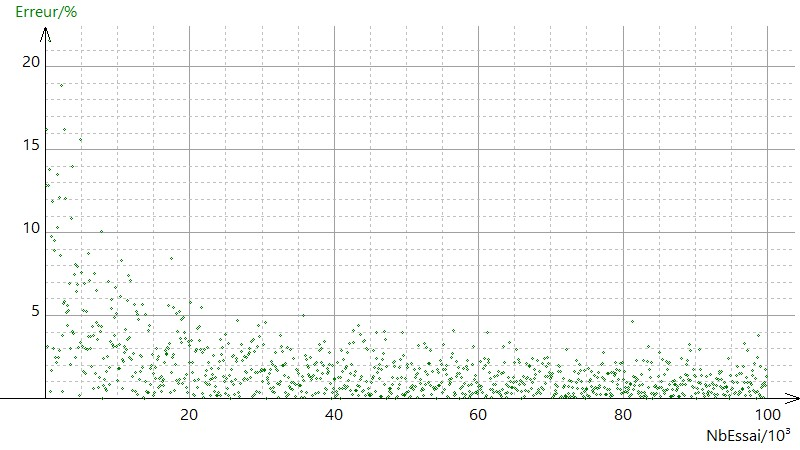
\includegraphics[width=\textwidth]{../graphe/Erreur3CR2L(n).jpg}
	\caption{Graphique de $Erreur=f(nbEssai)$ en variant $nbEssai$ de 100 à 100 000 par pas de 100}
\end{figure}	

\begin{figure}[H]
	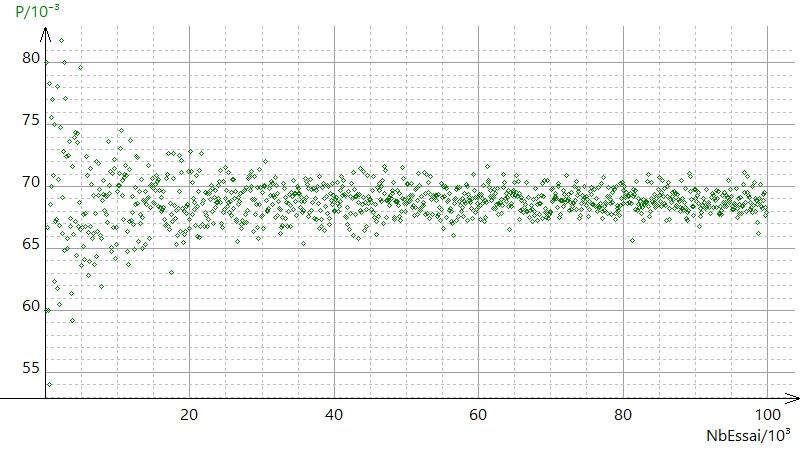
\includegraphics[width=\textwidth]{../graphe/P3CR2L(n).jpg}
	\caption{Graphique de $P=f(nbEssai)$ en variant $nbEssai$ de 100 à 100 000 par pas de 100}
\end{figure}	




\newpage
\section{Etude du cas E3C}
\subsection{Fonctions \textit{probaE3C} et \textit{trouverE3C}}

\begin{lstlisting}[language=java, caption={\it Fonction probaE3C et trouverE3C}, label=codeProbaE3C]
/**
 * FONCTION AJOUTEE
 * Action : Pour un paquet de 81 cartes distincts (3 Couleurs/ nbFiguresMax=3/ 3 Figures/ 3 Textures possibles par carte) : 
 * calcul experimentalement et retourne la frequence d'obtenir une Table (arrangement de 9 cartes distincts parmi les 81 du Paquet) contenant exactement 3 Cartes Rouges et 2 cartes ayant au moins 1 Losange.
 * Valeur theorique : non connue
 * @param nb nombre d'essai
 */
public static double probaE3C(int nb) {
    double countCasFavorable = 0;
    Paquet paq;
    for (int i = 0; i < nb; i++) {
        paq = new Paquet(
            Couleur.valuesInRange(0, 3), 
            3, 
            Figure.valuesInRange(0, 3), 
            Texture.valuesInRange(0, 3)
            );
        Carte[] tab = paq.piocher(9);
        if (trouverE3C(tab)) {
            countCasFavorable++;
        }    
    }
    return countCasFavorable;
}

/**
 * FONCTION AJOUTEE
 * Action : verifie si un ensemble de cartes contient un E3C
 * @param cartes
 * @return vrai si oui, false sinon;
 */
private static boolean trouverE3C(Carte[] cartes) {
    if (cartes.length < 3) {
        return false;
    }
    for(int i = 0; i < cartes.length; i++)
        for(int j = i+1; j < cartes.length; j++)
            for(int k = j+1; k < cartes.length; k++)
                if(Jeu.estUnE3C(new Carte[]{cartes[i], cartes[j], cartes[k]}))
                    return true;
    return false;
}
\end{lstlisting}


\newpage
\subsection{Traitements de données et analyse graphique}
\noindent De la même manière que pour les cas précédents, nous obtenons via une modélisation linéaire :

$$P_{E3C}exp = 0.70280 \pm 0.00011$$

\begin{figure}[H]
	\centering
	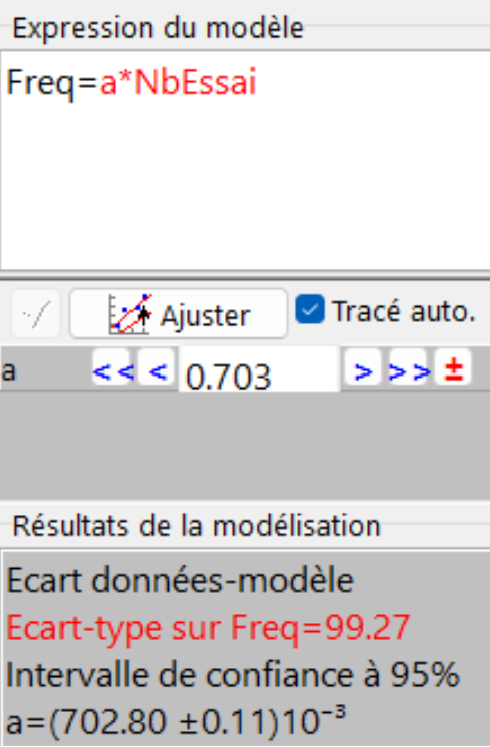
\includegraphics[scale=0.5]{../graphe/valDePE3C.png}
	\caption{Modélisation linéaire de $Freq(nbEssai)$ sur \textit{Regressi}}
\end{figure}

\begin{figure}[H]
	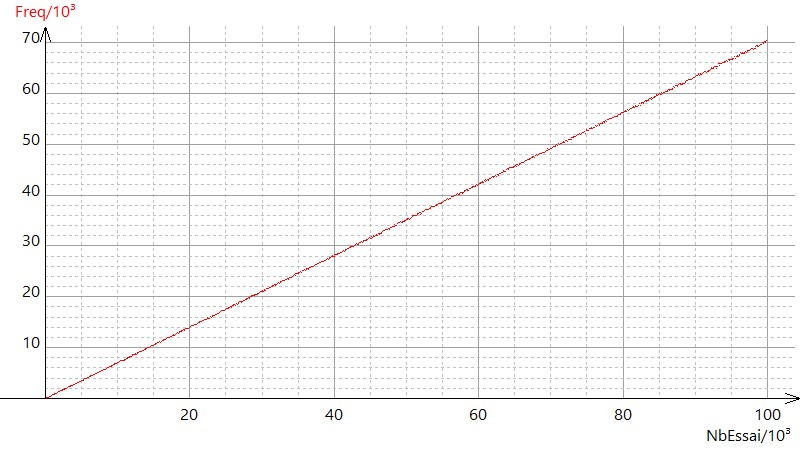
\includegraphics[width=\textwidth]{../graphe/FreqE3C(n).jpg}
	\caption{Graphique de $Freq=f(nbEssai)$ en variant $nbEssai$ de 100 à 100 000 par pas de 100}
\end{figure}	

\begin{figure}[H]
	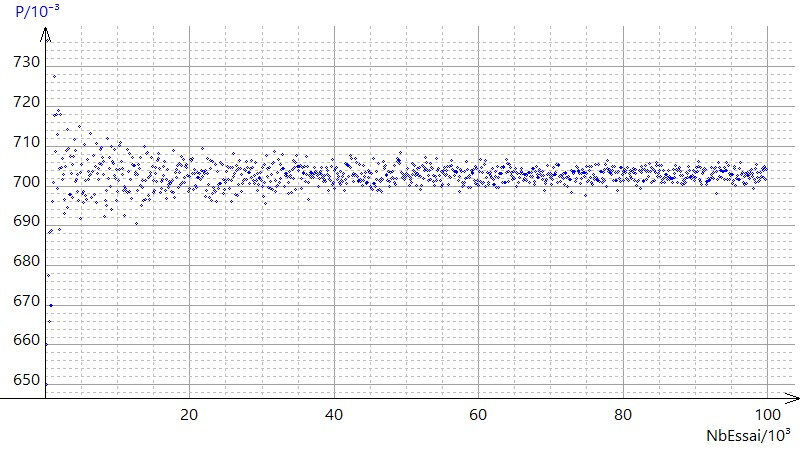
\includegraphics[width=\textwidth]{../graphe/PE3C(n).jpg}
	\caption{Graphique de $P=f(nbEssai)$ en variant $nbEssai$ de 100 à 100 000 par pas de 100}
\end{figure}	























\appendix
\chapter{Langages, IDE et logiciels utilisés}

\centering
  
\includegraphics[height=3.5cm]{../graphe/java.png}\qquad
  
\includegraphics[height=3.5cm]{../graphe/Vscode.png}\qquad
  
\includegraphics[height=3.5cm]{../graphe/idea.png} \qquad
  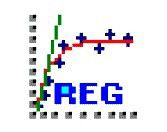
\includegraphics[height=3.5cm]{../graphe/regressi.jpg}
\centering

\end{document}









